% This is samplepaper.tex, a sample chapter demonstrating the
% LLNCS macro package for Springer Computer Science proceedings;
% Version 2.21 of 2022/01/12
%
\documentclass[runningheads]{llncs}
%
\usepackage[T1]{fontenc}
% T1 fonts will be used to generate the final print and online PDFs,
% so please use T1 fonts in your manuscript whenever possible.
% Other font encondings may result in incorrect characters.
%
\usepackage{graphicx}
% Used for displaying a sample figure. If possible, figure files should
% be included in EPS format.
%
% If you use the hyperref package, please uncomment the following two lines
% to display URLs in blue roman font according to Springer's eBook style:
\usepackage{color}
\usepackage{hyperref}
\renewcommand\UrlFont{\color{blue}\rmfamily}
\urlstyle{rm}

\usepackage{graphicx}
\usepackage{subcaption}

\usepackage{amsmath}

%
\begin{document}
%
\title{Benchmarking Automatic License Plate Recognition: Dataset Collection and Performance Evaluation}
%
\titlerunning{Benchmarking ALPR}
% If the paper title is too long for the running head, you can set
% an abbreviated paper title here
%
\author{Oskar Bełza \and
Wojciech Górecki \and
Konrad Kuś \and
Dawid Mrówczyński \and
Jakub Szczepański \and
Mikołaj Golański\and
Piotr Stefański\orcidID{0000-0003-1229-327X}}
%
\authorrunning{Oskar Bełza et al.}
% First names are abbreviated in the running head.
% If there are more than two authors, 'et al.' is used.
%
\institute{Student research group of algorithmics and programming, University of Economics in Katowice, 1 Maja 50, 40-287 Katowice, Poland
\email{oskar.belza@edu.uekat.pl}
}
%
\maketitle              % typeset the header of the contribution
%
\begin{abstract}

Automatic License Plate Recognition (ALPR) has become a crucial technology in domains such as traffic monitoring, toll collection, and security enforcement. This study compares traditional image-processing methods, YOLO-based deep learning algorithms, HOG-based feature extraction, and convolutional neural networks (CNNs) to give a full picture of ALPR systems. The study involves putting together a set of 195 real-life pictures of car license plates and trying out different ways to recognize them. The results of the experiment show that the modified YOLO-based method is the most accurate (65.64\%) and also processes data quickly. On the other hand, character misclassification and processing speed are issues for conventional image processing, HOG-based methods, and CNN-based strategies. This study discusses the advantages and disadvantages of each approach and demonstrates that ALPR can still be improved in the area of operating in unidentified conditions.

\keywords{Automatic License Plate Recognition \and Dataset Collection \and Benchmarking \and Computer Vision \and Deep Learning}
\end{abstract}
%
%
%

\section{Introduction}

Automatic License Plate Recognition (ALPR) systems are an important part of modern smart transportation systems. Traffic monitoring, toll collection, parking management, and law enforcement all use them a lot. The main job of an ALPR system is to find license plates in pictures or video streams and correctly read their alphanumeric content in real time.

Recent improvements in computer vision and machine learning have made ALPR work a lot better. But it's still hard to get consistent accuracy in real-world situations that aren't controlled. Detection and recognition accuracy can suffer from things like changing lighting, plates that are at an angle, obstructions, and regional plate formats. Deep learning methods need big, varied datasets and a lot of computing power, while traditional image-processing methods don't always work in these kinds of situations.

In this study, we focus on evaluating the generalization capabilities of several ALPR techniques when applied to unfamiliar data. To do this, we made our own dataset of 195 license plate pictures taken on a university campus in real life. This dataset was made to have different angles, lighting conditions, and backgrounds to show how complicated real-world deployments can be.

We test four methods—traditional image processing, Histogram of Oriented Gradients (HOG), Convolutional Neural Networks (CNNs), and YOLO-based object detection—against strict criteria like full string accuracy and processing time. We want to try these methods on new data to see how well they work, where they don't work, and what else we can do to make ALPR systems more flexible and reliable.


\section{Related works}

Because they are used for traffic monitoring, toll collection, and security, Automatic License Plate Recognition (ALPR) systems have gotten a lot of attention. Researchers have been working on making them more accurate, efficient, and strong in a variety of situations. This part gives a quick overview of the most important contributions to preprocessing, plate localization, character segmentation, and recognition.

The first system splits ALPR into plate localization using fuzzy logic and character recognition via neural networks. It achieved 97.9\% detection and 95.6\% recognition success, with an overall rate of 93.7\%~\cite{chang2004automatic}.

Another system follows steps including preprocessing, plate extraction, character segmentation, and Euclidean template matching, with extra care for similar characters (e.g., '8' vs. 'B'). It is both fast and accurate~\cite{shi2005automatic}.

A location-specific approach reviews ALPR methods using a dataset of Ontario vehicles, addressing regional format differences~\cite{ahmad2015automatic}.

One study uses YOLO and fine-tuned CNNs with data augmentation. It reached 93.53\% recognition at 47 FPS on SSIG and 78.33\% on a larger dataset, outperforming commercial systems~\cite{laroca2018robust}.

Another work employs deep CNNs and spatial transformer networks (STN) to handle diverse plate formats and video conditions, demonstrating strong performance~\cite{jain2016deep}.

A survey contrasts multi-stage (detection, segmentation, recognition) and single-stage (deep learning) ALPR systems. While deep models achieve high accuracy, they require significant computational power and struggle in low-light conditions~\cite{9310202}.

An alternative method integrates Faster R-CNN, morphological processing, and deep learning. Tested on PKU, AOLP, and CCPD datasets, it achieved recognition rates of 99\%, 96.02\%, and 98.7\%, respectively~\cite{app13063956}.

Another review examines methods like Otsu thresholding, Sobel edges, and CNN-based segmentation. Combined with OCR and SVMs, accuracy can reach up to 99.5\%, though performance varies with lighting and plate quality~\cite{s21093028}.

A comparison of EasyOCR and TesseractOCR with YOLOv5 shows EasyOCR achieving 95\% accuracy and better numeric recognition, while Tesseract performs slightly better with alphabetic characters~\cite{10009215}.

The final work introduces a multinational ALPR system using tiny YOLOv3, YOLOv3-SPP, and layout detection. It handles single- and double-line formats, achieving high accuracy across plates from 17 countries~\cite{9003211}.


\section{Methodology}
\label{sec:methodology}
This section talks about the methods used to create and test Automatic License Plate Recognition (ALPR) systems. The first step was to gather a wide range of images of vehicle license plates taken on the university campus in real life. Next, there was a review of the literature that looked at both traditional image processing methods and newer ones based on deep learning.

This paper gives an overview of different ALPR algorithms, from older ones to newer ones like convolutional neural networks and frameworks for detecting objects in real time. We used standardized performance metrics to make sure that the evaluation was fair and consistent. Accuracy and processing time were two of the most important factors for real-time ALPR deployment.


\subsection{Data Collection on Campus}

To support the evaluation of Automatic License Plate Recognition (ALPR) algorithms, a dataset was collected at two parking lots near the entrance of the \textit{CNTI building} on our university campus (\textbf{1 Maja 50, 40-287 Katowice, Poland; 50.260488 N, 19.045213 E}). These locations allowed us to collect a diverse set of data in real-life conditions. Their positions are marked on the campus map (Fig.~\ref{fig:cnti_map}).

\begin{figure}[ht]
    \centering
    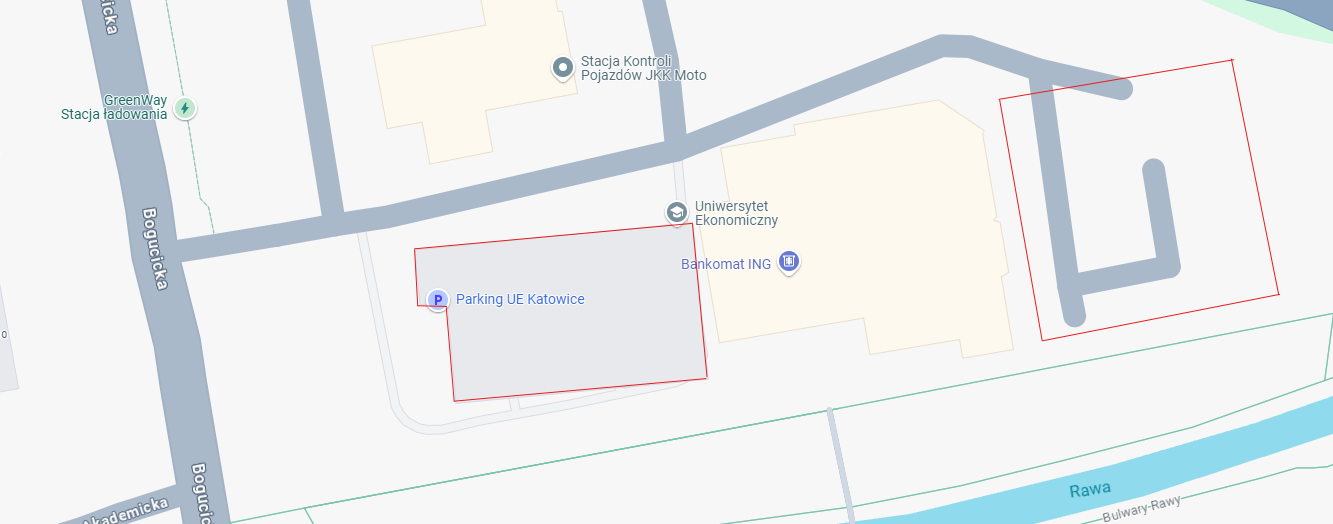
\includegraphics[width=0.8\linewidth]{images/CNTI.png}
    \caption{Map showing the two parking lots used for ALPR dataset collection near the CNTI building.}
    \label{fig:cnti_map}
\end{figure}

\paragraph{Setup and Equipment}
High-resolution smartphones (\textit{XIAOMI Redmi Note 9 Pro} and \textit{iPhone 13 Pro}) were used to capture license plates. Two setups were applied for diverse viewpoints.

In the first, the camera was mounted on a tripod at a height of \textbf{30 cm}, directly facing incoming vehicles at a \textbf{0°} angle to capture clear frontal images (Fig.~\ref{fig:setup_example}). In the second, the camera was placed on the hood of a nearby parked car, providing a slightly elevated, angled perspective to test recognition under varied spatial conditions (Fig.~\ref{fig:setup_vehicle}).


\begin{figure}[ht]
    \centering
    \begin{subcaptionbox}{Tripod-mounted camera at 30 cm, facing incoming vehicles.\label{fig:setup_example}}[0.45\linewidth]
        {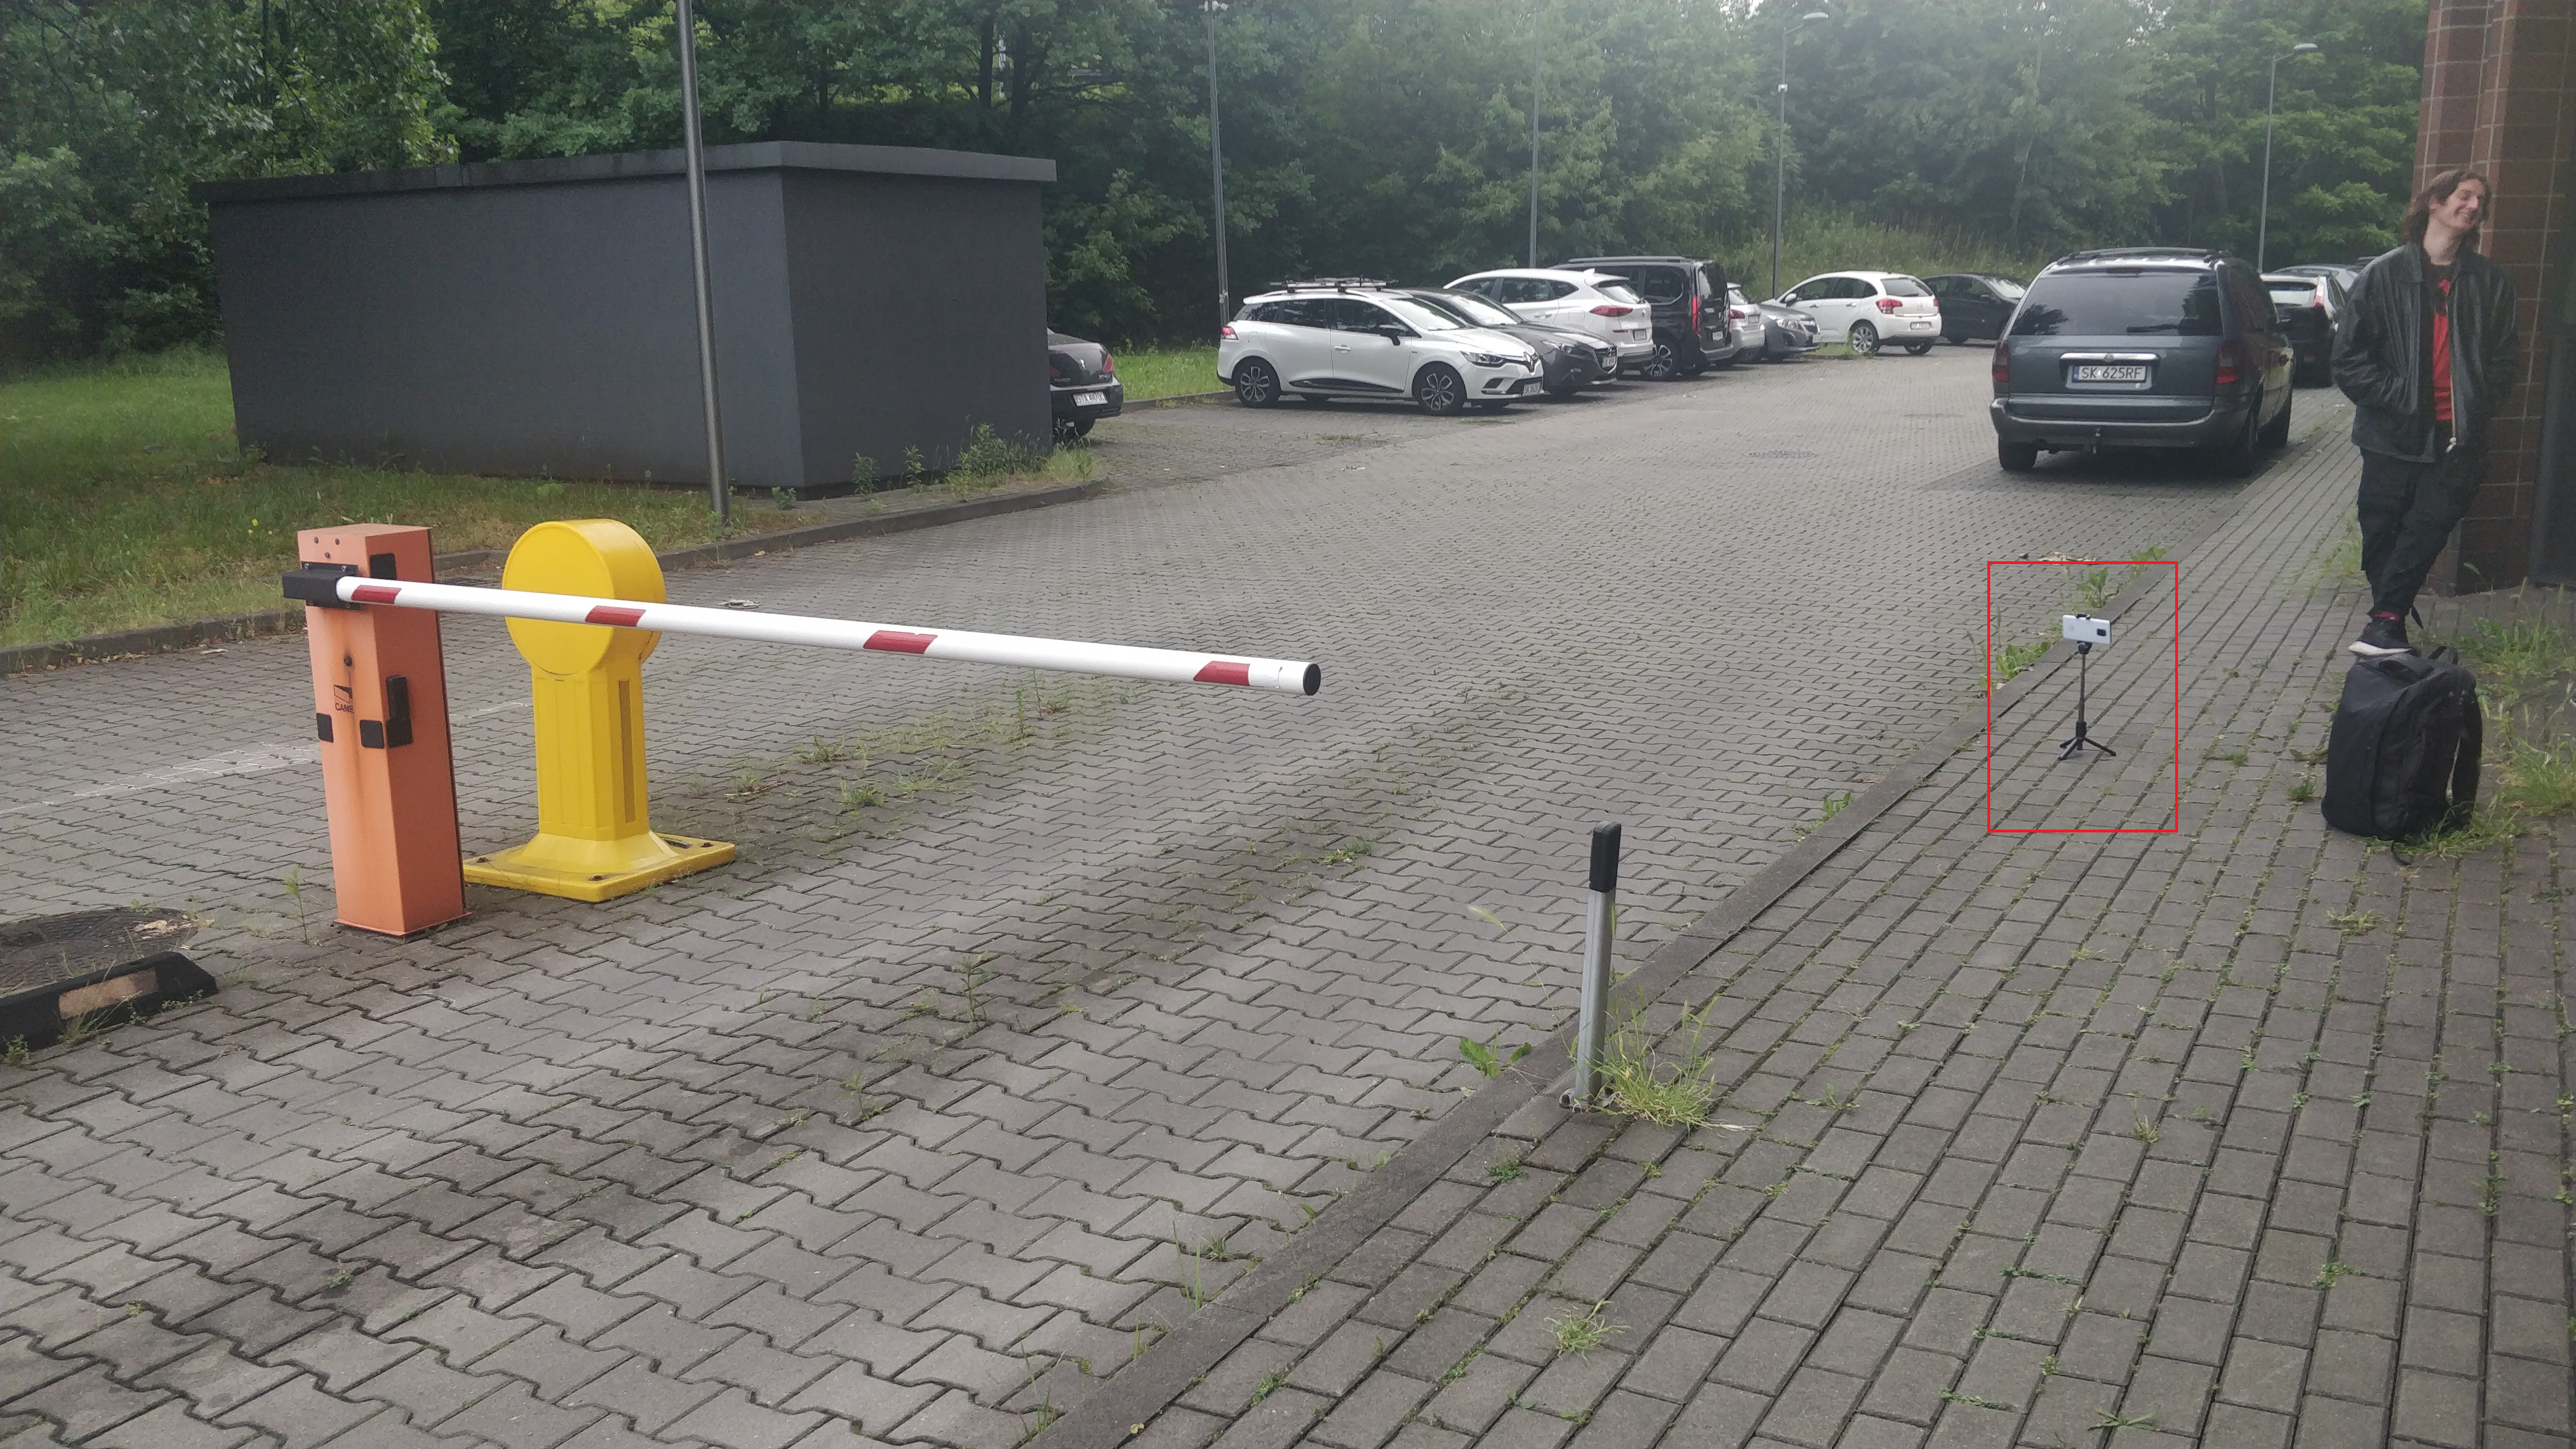
\includegraphics[width=\linewidth]{images/stanowisko_1.png}}
    \end{subcaptionbox}
    \hfill
    \begin{subcaptionbox}{Camera on the hood of a parked vehicle, capturing from an alternative angle.\label{fig:setup_vehicle}}[0.45\linewidth]
        {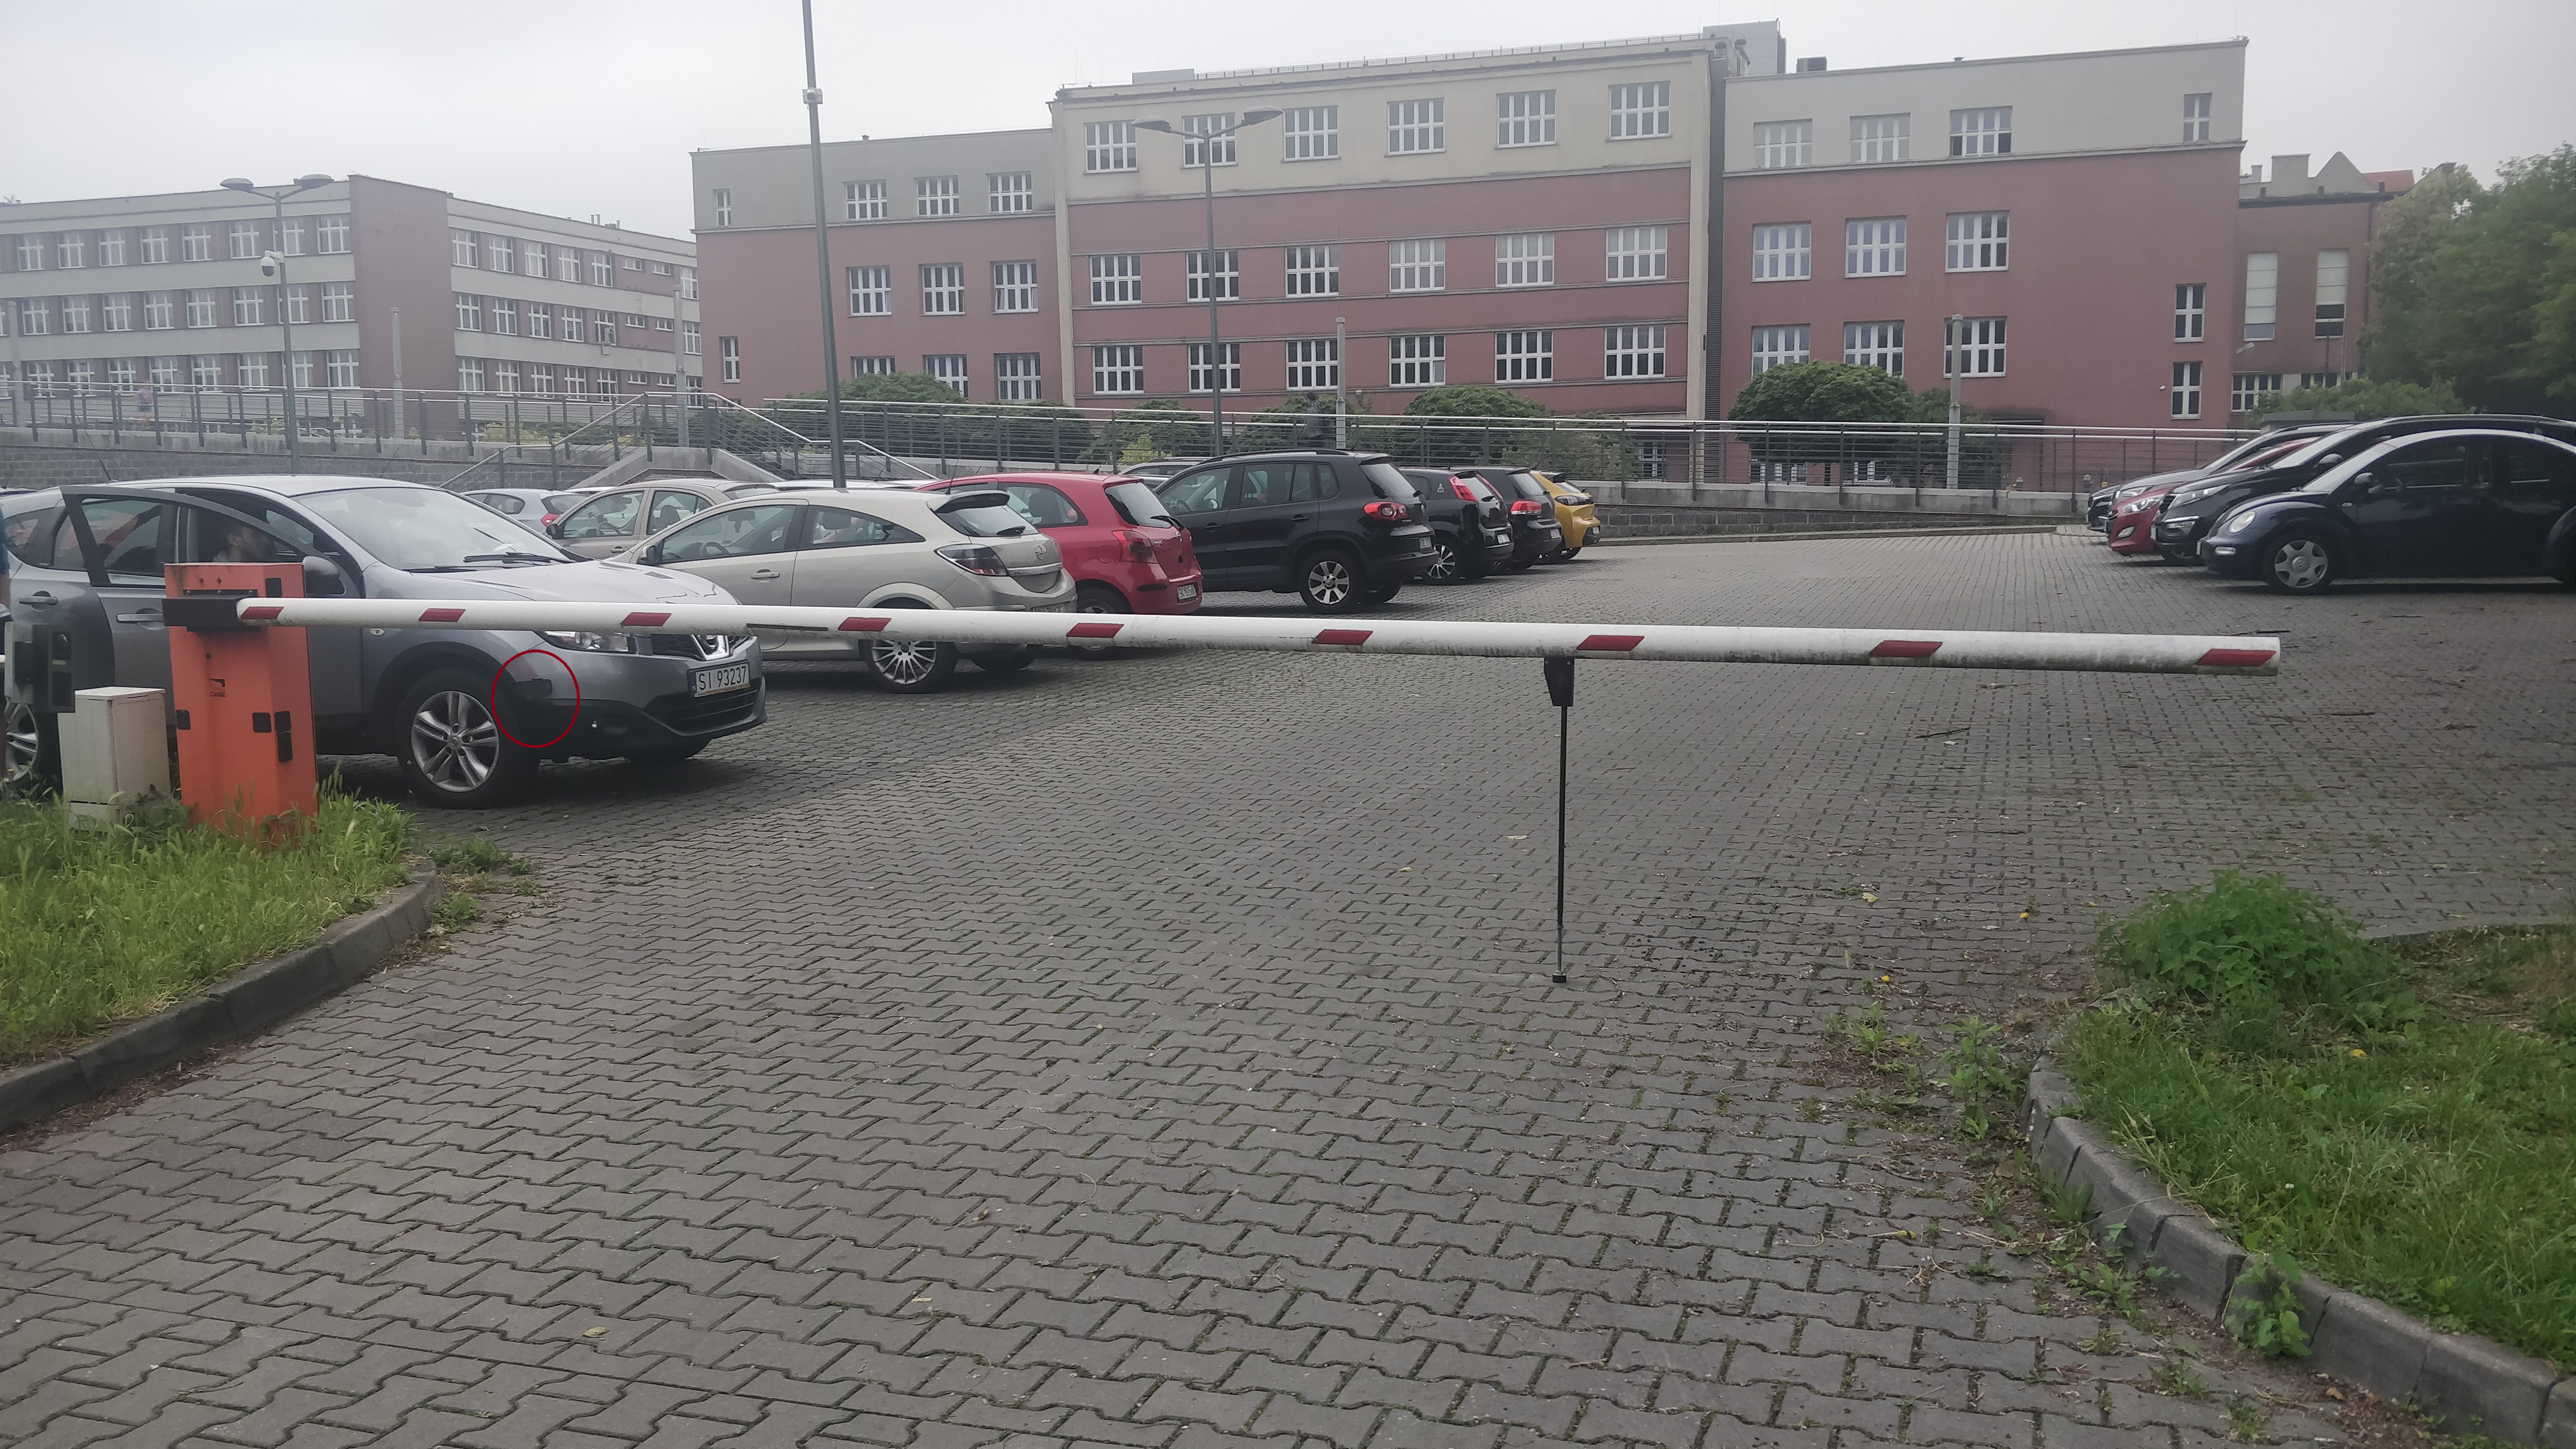
\includegraphics[width=\linewidth]{images/stanowisko_2.png}}
    \end{subcaptionbox}
    \caption{Two different camera setups used for ALPR dataset collection near the parking lot entrance.}
    \label{fig:camera_setups}
\end{figure}


\paragraph{Dataset Overview}
The final dataset includes pictures taken in controlled but real-world situations, with different weather and lighting conditions. The distance between the vehicles and the camera was between 1 and 2 meters. The goal of this setup was to mimic typical ALPR situations that happen in the real world, like keeping an eye on parking lots or gated entry systems.

Different weather conditions were used to take pictures so that they would work in different environments. For example, Fig. \ref{fig:sunny_example} shows a picture of a car's license plate taken on a sunny day, which makes it hard to see because of glare and reflections. Figure \ref{fig:cloudy_example}, on the other hand, shows a picture taken on a cloudy day, when the lighting is more even but may make the contrast and sharpness less clear.

\begin{figure}[ht]
    \centering
    \begin{subcaptionbox}{Sunny day\label{fig:sunny_example}}[0.45\linewidth]
        {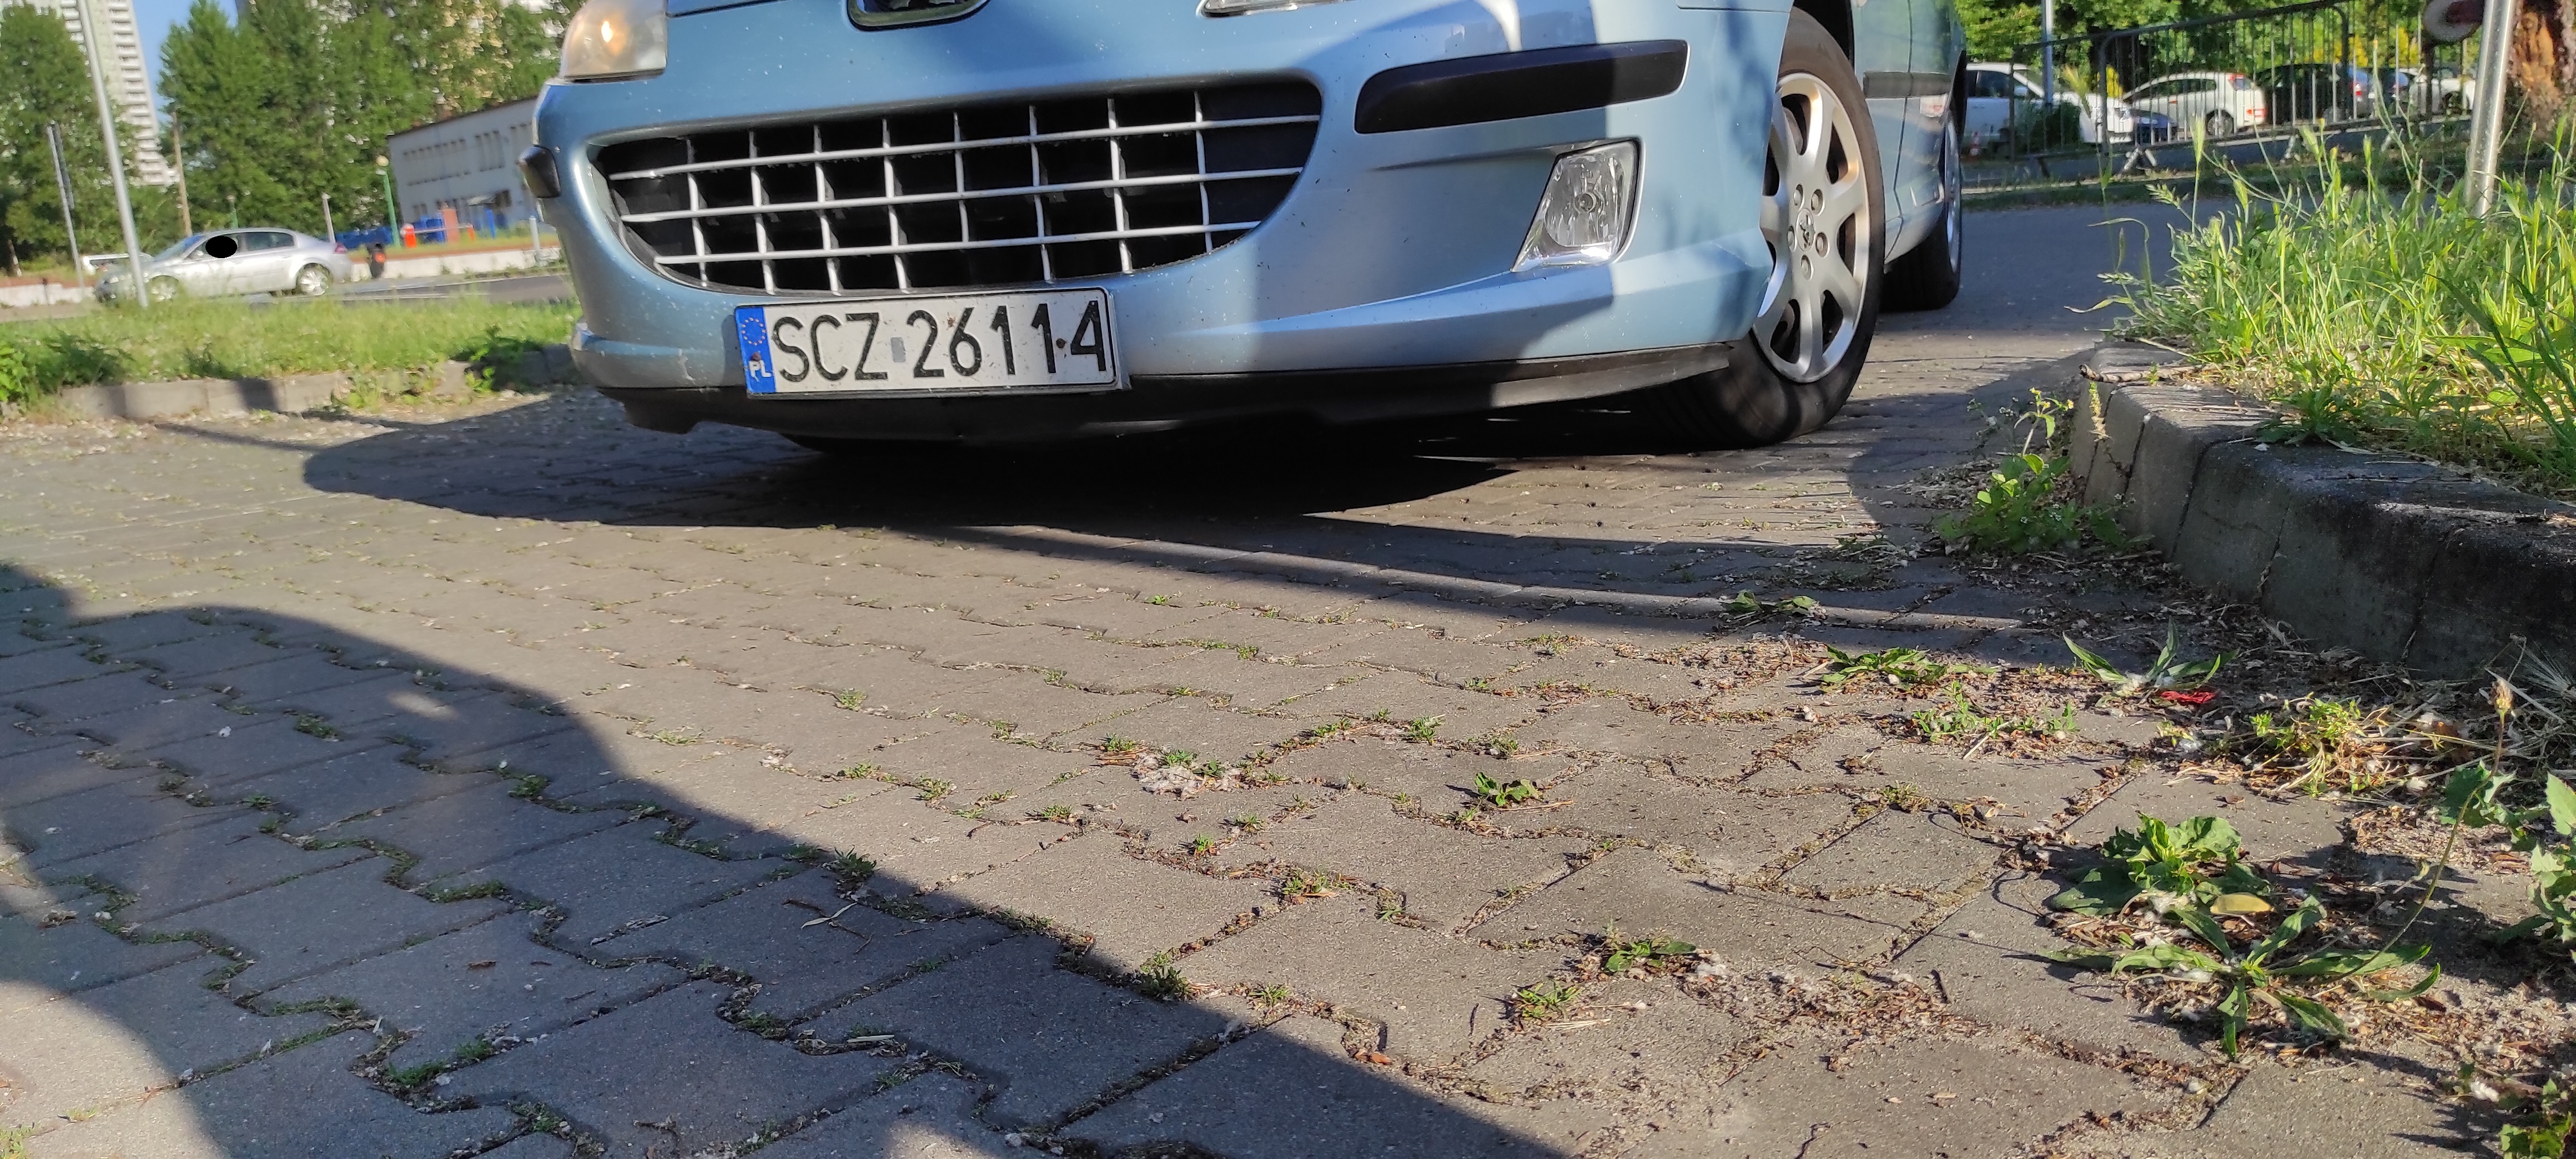
\includegraphics[width=\linewidth]{images/przykład_1.jpg}}
    \end{subcaptionbox}
    \hfill
    \begin{subcaptionbox}{Cloudy day\label{fig:cloudy_example}}[0.45\linewidth]
        {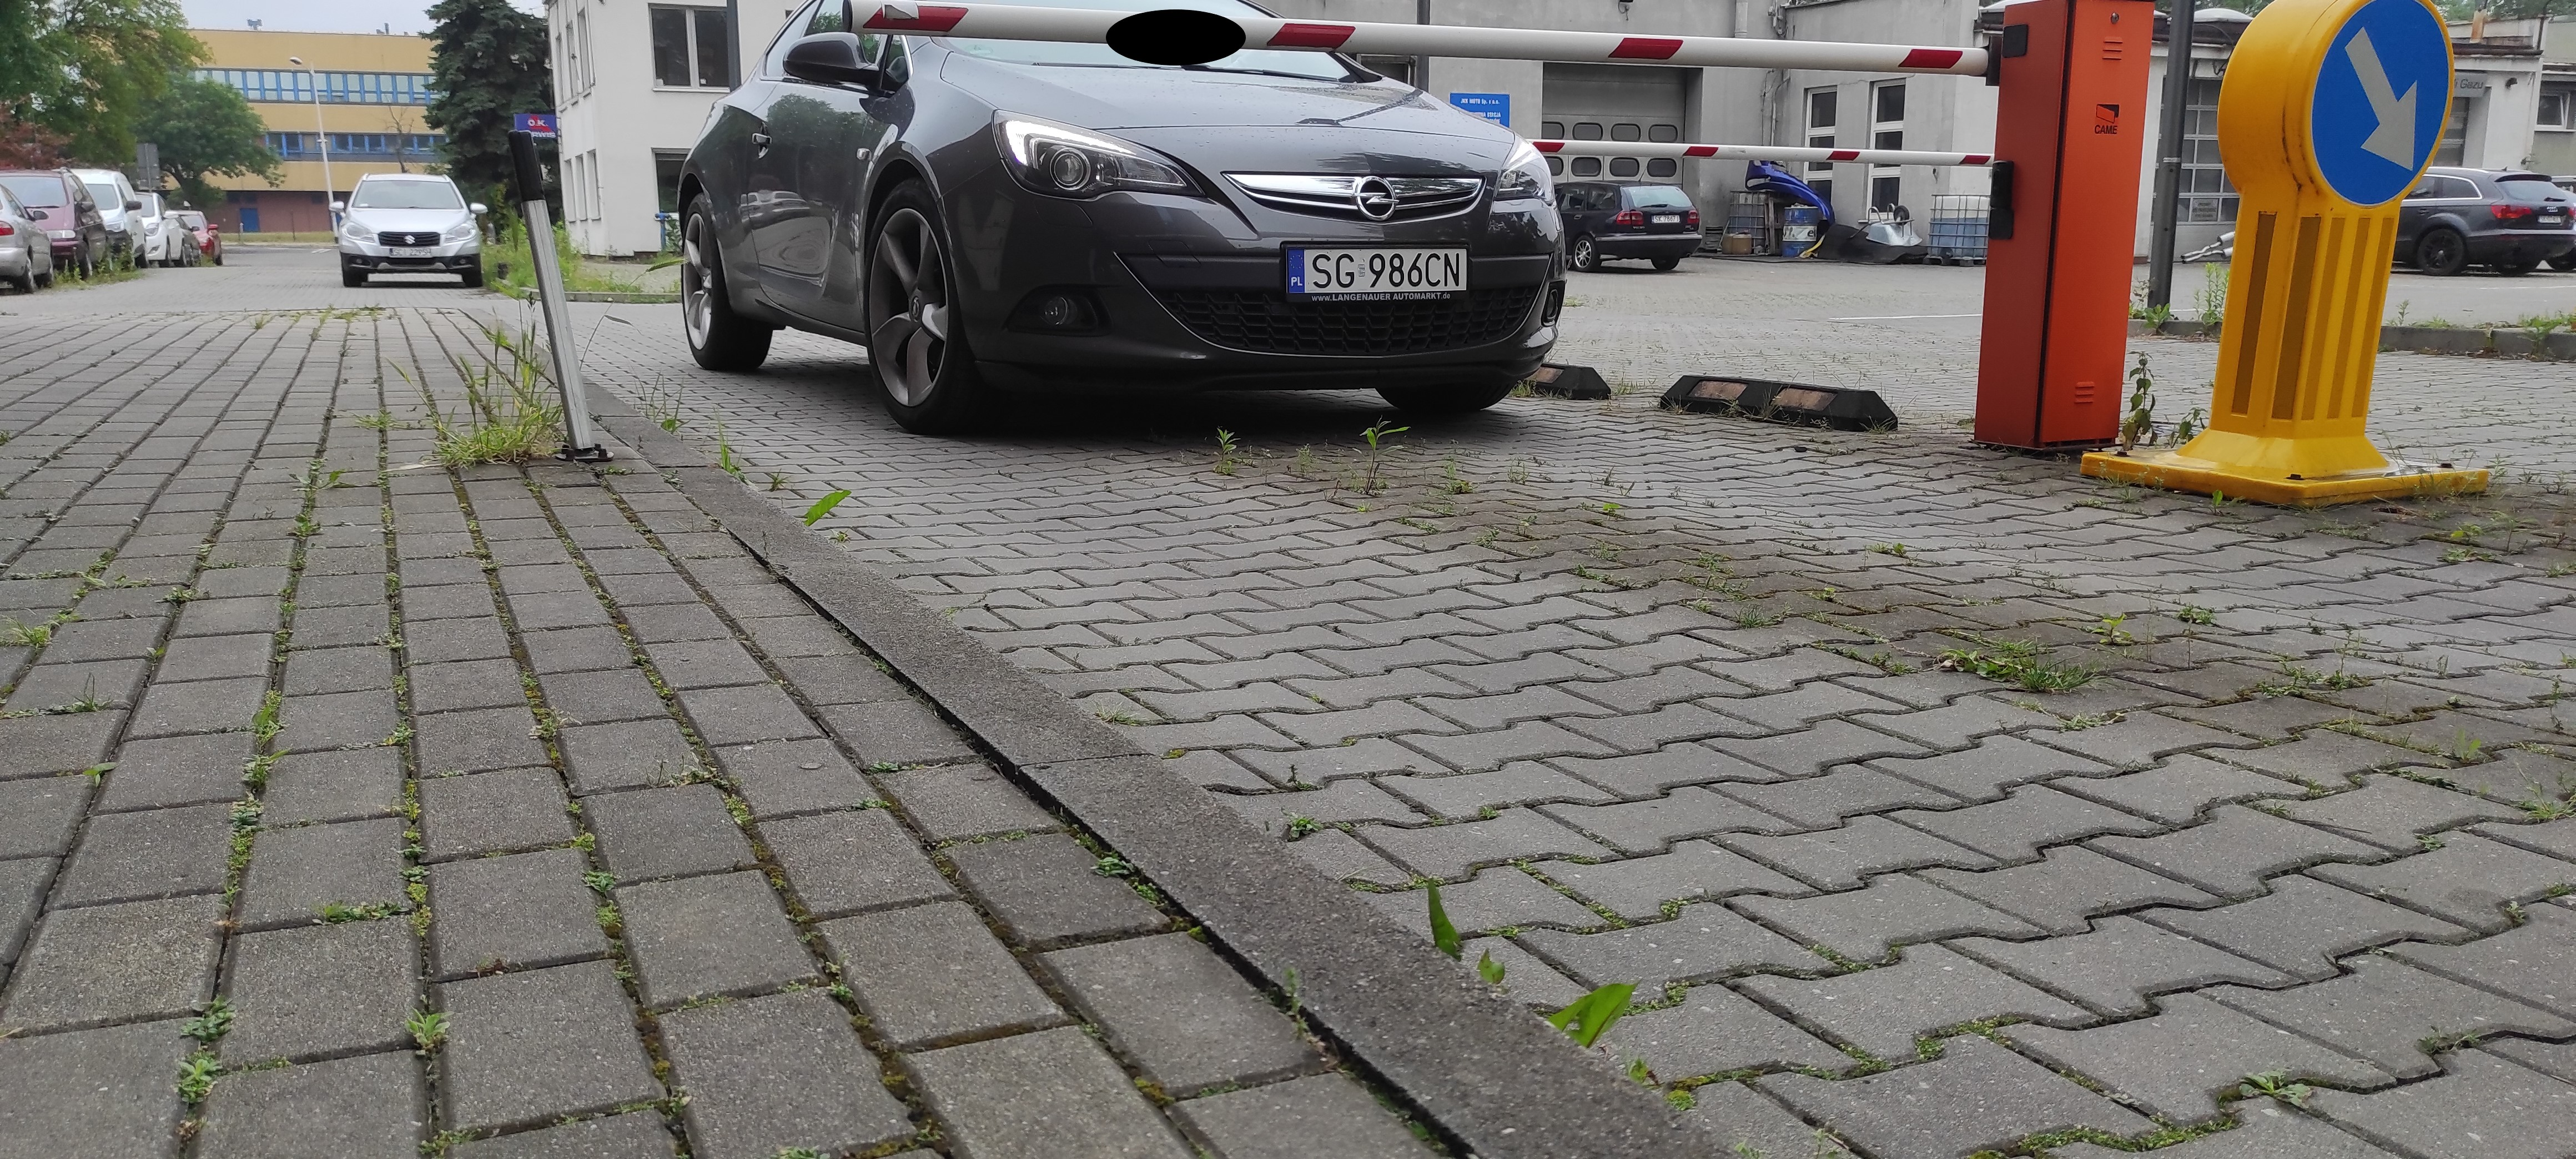
\includegraphics[width=\linewidth]{images/przykład_2.jpg}}
    \end{subcaptionbox}
    \caption{Sample images of vehicle license plates captured in different weather conditions.}
    \label{fig:weather_examples}
\end{figure}

\paragraph{Data Availability}  
You can find the full dataset, which includes 195 images taken in different situations, on Kaggle at the following link: \url{https://www.kaggle.com/datasets/piotrstefaskiue/poland-vehicle-license-plate-dataset} as of May 20, 2025. There are a lot of real-world examples in this dataset that can be used to see how well different ALPR algorithms work in different kinds of weather.


\subsection{Overview of Algorithms for Automatic License Plate Recognition (ALPR)}  
ALPR systems use different methods to find and read license plates. These methods range from old-fashioned image processing to new deep learning methods:

\begin{enumerate}
    \item \textbf{Classical Image Processing Techniques:}  
    These rely on basic image analysis steps:
    \begin{itemize}
       	\item \textit{Preprocessing:} Changing the color to gray and getting rid of noise.
\item \textit{Finding Edges:} Canny and Sobel are two methods that find areas with a lot of contrast.
\item \textit{Thresholding:} Otsu's method and other techniques binarize the image.
\item \textit{Segmentation:} Morphological operations separate the plate and the characters.
    \end{itemize}
    While efficient, these methods struggle with poor lighting, occlusion, or non-standard plates.

    \item \textbf{Histogram of Oriented Gradients (HOG):}  
    HOG gets gradient-based features from small image cells and then normalizes them over blocks. When used with classifiers like SVM, it can find characters, but it is less reliable when there are a lot of distortions.

    \item \textbf{Convolutional Neural Networks (CNN):}  
    CNNs automatically learn visual features for both plate detection and character recognition:
    \begin{itemize}
        \item \textit{Feature Extraction:} From low-level edges to high-level patterns.
        \item \textit{Detection and Recognition:} Localize plates and classify characters.
    \end{itemize}
    CNNs are effective under challenging conditions but require large datasets and high computational power.

    \item \textbf{YOLO (You Only Look Once):}  
    A real-time detection algorithm that:
    \begin{itemize}
        \item \textit{Processes the entire image in one pass,}
        \item \textit{Uses grid-based object localization,}
        \item \textit{Detects multiple objects simultaneously.}
    \end{itemize}
    YOLO is great for live traffic systems because it can quickly and accurately find things. However, it may need to be adjusted for small or far-away plates..
\end{enumerate}

In short, classical methods are easy to use and quick, but CNNs and YOLO work better in changing, real-world situations.


\subsection{Selection of Performance Metrics}
A set of standardized evaluation metrics was chosen to systematically compare how well each algorithm worked. Efficiency and processing time were given special attention because ALPR systems need to work in real time. Some important metrics are:

\begin{enumerate}
    \item \textbf{Accuracy} evaluates a model's ability to locate license plates. It is defined as the proportion of accurate predictions to all predictions:

    \begin{equation}
        \text{Accuracy} = \frac{\text{Number of Correct Predictions}}{\text{Total Number of Predictions}} \times 100\%
    \end{equation}

    A prediction is correct when the recognized plate matches the ground truth perfectly, with all letters and symbols. A wrong character (like confusing \texttt{O} with \texttt{0}) will make the prediction wrong.

    \begin{itemize}
        \item \textbf{Correct:} \\
        Actual: \texttt{ABC1234} \\
        Predicted: \texttt{ABC1234}
        
        \item \textbf{Incorrect:} \\
        Actual: \texttt{ABC1234} \\
        Predicted: \texttt{ABC1334}
    \end{itemize}

    \item \textbf{Processing time} measures the time it takes for an image to be recognized. We take the average of 10 runs to make sure that the results are repeatable. In our case, we measure how long it takes to process our entire dataset of 195 images. This metric is very important for real-world uses like monitoring traffic, collecting tolls, or finding cars on watchlists.

We prefer algorithms that take less time to process because they let things run quickly and without delays. Good performance makes sure that the system can handle a lot of traffic and respond quickly in changing situations.
\end{enumerate}


\section{Experiments}
\label{sec:experiments}

We used a set of license plate images that met local standards to run a series of tests to see how well Automatic License Plate Recognition (ALPR) algorithms worked. 

Four methods were used to evaluate: a traditional image-processing method, a HOG-based method, a YOLO-based machine learning model (with and without changes), and a Convolutional Neural Network (CNN)-based model.

\subsection{Classical Image-Processing Approach}
The first approach relied on traditional image processing techniques to locate license plates and recognize characters. The procedure included:
\begin{enumerate}
    \item Grayscale conversion,
    \item Noise reduction using Gaussian blur,
    \item Canny edge detection,
    \item Contour detection and sorting by area,
    \item Polygonal approximation to find rectangular shapes,
    \item Region of interest (ROI) masking and cropping,
    \item OCR-based recognition using Tesseract.
\end{enumerate}

This method achieved an accuracy of 15.38\% and an average execution time of 69.12 seconds for the full dataset (195 images). A common issue was confusion between visually similar characters. Accuracy was evaluated using a strict binary criterion: even a single incorrect character resulted in a failed prediction ~\cite{kagglePlateNumber}.

\subsection{HOG-Based Approach}
The second approach used a pre-trained Support Vector Machine (SVM) classifier along with Histogram of Oriented Gradients (HOG) features. Size-based contours were extracted and filtered. HOG features were then calculated and categorized. The cropped plate area was sent to Tesseract OCR for regions that were positively identified.

Nine orientation bins, $9\times9$ pixel cells, and $3\times3$ cell blocks were used to extract HOG features. Resizing, grayscale conversion, adaptive thresholding, and morphological operations were all part of the preprocessing pipeline.

With an average processing time of 93.74 seconds, this method achieved 16.92\% accuracy. Character confusion and incorrect region-of-interest (ROI) selection remained problems, even though it performed marginally better than the classical method ~\cite{SardhenduMishraHOG}.

\subsection{YOLO-Based Approach}

The YOLO (You Only Look Once) algorithm was evaluated in two configurations:

\begin{itemize}
    \item \textbf{With Modifications:} The model took an average of 107.88 seconds to process and was 65.64\% accurate after being modified to fit local license plate formats.
    
    \item \textbf{Without Modifications:} The original YOLO implementation, which was trained on Pakistani plates, was only 22.05\% accurate and took 115.88 seconds to process.
\end{itemize}

The fact that there were past processing steps that were only for Pakistani plate standards was a big problem with the unmodified version. The original code, in particular, had logic that changed the order of plate numbers to fit the formatting rules in each area. This change didn't work with our data set, so we had to make a second scenario that clearly stopped this behavior. By turning off this transformation and changing the model's post-processing logic, we put the recognized characters back in the order they naturally go in. This made the results match local plate conventions.

The changed YOLO setup did much better than any other method, both in terms of speed and accuracy. Partial occlusions, on the other hand, hurt performance in both situations because YOLO needs to correctly detect vehicles before it can find plates ~\cite{usama2022vehicle}.


\subsection{CNN-Based Approach}
We only used the CNN-based method to find license plates, and then we used OCR to read the characters. It took 292.32 seconds to process the whole dataset and got an accuracy of 7.18\%. 

One big problem with this method was that it was hard to find license plates in the pictures accurately. A lot of the time, incorrect or imprecise bounding boxes caused cropped areas that didn't fully include the plate or had backgrounds that weren't relevant. This made the next OCR stage much less effective. The strict evaluation criterion, which required an exact match, had an effect on the final accuracy, just like in other approaches ~\cite{githubGitHubArtisan1218AutomaticLicensePlateReader}. 


\subsection{Comparison of Results}
We used a benchmark made for this project to compare all of the methods in terms of accuracy and speed of execution. This benchmark, which can be found on GitHub, makes sure that all ALPR methods are tested in the same way. You can get to the repository at \href{https://github.com/WojteGK/license-plate-recognition-benchmark}{GitHub repository} as of May 20, 2025. Table~\ref{tab:results} shows a summary of the results.


\begin{table}[ht]
    \centering
    \caption{Comparison of Detection Approaches for License Plate Recognition}
    \label{tab:results}
        \begin{tabular}{|l|c|c|c|}
        \hline
        \textbf{Method} & \textbf{Accuracy} & \textbf{Execution Time (s)} \\
        \hline
        Classical Approach & 15.38\% & 69.12 \\
        \hline
        HOG-Based Approach & 16.92 & 93.74 \\
        \hline
        YOLO (With Modifications) & 65.64\% & 107.88 \\
        \hline
        YOLO (Without Modifications) & 22.05\% & 115.88 \\
        \hline
        CNN-Based Approach & 7.18\% & 292.32 \\
        \hline
        \end{tabular}
\end{table}

\subsection{Testing Environment}
The approaches were tested on a system with the following specifications:
\begin{itemize}
    \item \textbf{Hardware:} AMD Ryzen 7 7745HX with Radeon Graphics, 16GB RAM
    \item \textbf{Software:} Windows 10 x64
    \item \textbf{Python Versions:} 
        \begin{itemize}
            \item Classical Approach: Python 3.12.4,
            \item HOG Approach: 3.12.4,
            \item YOLO (Both Versions): Python 3.6.8,
            \item CNN-Based Approach: Python 3.10.
        \end{itemize}
    \item \textbf{Dataset:} Locally collected dataset of 195 license plate images.
\end{itemize}

We measured accuracy by counting the number of license plates that were correctly identified. We used a strict binary evaluation, which meant that even one wrong character meant that the recognition was marked as a failure. The execution time is the average time it takes to process one out of ten iterations, which includes all 195 images.

\subsection{Summary}

The results of the evaluation clearly show that the YOLO-based method with local changes is better than other methods in both accuracy and speed of processing. With an accuracy of 65.64\% and a reasonable execution time, it is the best choice for real-time ALPR applications.

The classical and CNN-based methods, on the other hand, were much less accurate, with rates of 15.38\% and 7.18\%, respectively. It was hard for them to tell which characters were which when they looked alike. The HOG-based method only made the classical method a little better, with an accuracy of 16.92\%, but it also added more computation time.

These results show how important it is for algorithms to be flexible and to use data that is specific to the field. Local tuning of detection models, like YOLO, makes them work much better than ready-made ones.

\section{Conclusions}

This study showed four ALPR methods using data from the real world. The YOLO-based method with local changes turned out to be the best, with a good balance between speed and accuracy. Other methods, like classical, HOG-based, and CNN-based, had problems with character-level misclassification and were sensitive to the quality of the images.

One important finding is that models that do well on benchmark datasets often don't work well in real life. This shows how important it is to make changes that are specific to the domain, such as better preprocessing and fine-tuning on local datasets. Character misclassification, changes in lighting, and the limits of the dataset are still big problems.

To make sure that ALPR works well in changing environments, future research should focus on making it more robust by using adaptive preprocessing, better OCR models, and more general training datasets.


%
% ---- Bibliography ----
%
% BibTeX users should specify bibliography style 'splncs04'.
% References will then be sorted and formatted in the correct style.
%
\bibliographystyle{splncs04}
\bibliography{mybibliography}
%

\end{document}
